\documentclass{article}     
\usepackage[utf8x]{inputenc}
\usepackage[english,russian]{babel}
\usepackage{upgreek}
\usepackage{graphicx}
\usepackage{wrapfig}
\usepackage{amsmath}
\graphicspath{{images/}}


\begin{document}
\begin{titlepage}
\begin{center}
{\bf САНКТ-ПЕТЕРБУРГСКИЙ ГОСУДАРСТВЕННЫЙ УНИВЕРСИТЕТ\\
МАТЕМАТИКО-МЕХАНИЧЕСКИЙ ФАКУЛЬТЕТ\\}
\end{center}

\vspace{2cm}
 \begin{center}
  \Huge{\bf{Построение профилей линий в спектрах
   звезд\\ типа 
   $\uptau$Tau и Ae/Be Хербига }}
 \end{center}

\vspace{2cm}

\large
 \hspace{8cm}\parbox{8cm}{	

{\bf Курсовая работа}\\
студента 391 группы\\
Д.В.\,Дмитриева  
\vspace{1cm}

{\bf Научный руководитель}\\
 д.ф.-м.н, профессор РАН\\ В.П.\,Гринин \\ 
}

\vfill 
\begin{center}
Санкт-Петербург

2016
\end{center}

\end{titlepage}
\newpage
\tableofcontents
\newpage

\numberwithin{equation}{section}


\section{Введение}



В данной работе на основе метода Соболева \cite{sobolev47} для сред с большими градиентами скорости разработан алгоритм для численного моделирования 
профилей эмиссионных линии, наблюдаемых в спектрах звезд типа Т Тельца и Ae/Be Хербига. 
Это молодые звезды, ещё не достигшие главной последовательности. Они отличаются массами, эффективной темпертарурой и скоростями вращения: 
звезды типа Т Тельца ($Т_{ef} \approx$ 4000 K) имеют массы в интервале от 0.2 до 2 $M_\odot$; их средняя скорость вращения равна примерно 15 км/с 
(см. обзор Петрова \cite{petrov}.). Звезды АеВе Хербига имеют более высокие эффективные температуры ($T_{ef} \approx$ 8000-30000 K). 
Их массы заключены в пределах от 2 до 10 $M_\odot$. Скорости вращения достигают значений порядка 100-200 км/с (см. обзор \cite{waters98}).
     
\begin{equation}
\sqrt{1+y'^2} = \frac{y'}{\sqrt{1+y'^2}} (y' - f_1')\mid_{x=x1}
\end{equation}

\begin{equation}
1+y'^2 = y' (y' - f_1')\mid_{x=x1}
\end{equation}

\begin{equation}
0 = \frac{3c^3}{4} + \frac{3c}{2} - \frac{1}{2c^2}
\end{equation}

\begin{equation}
\begin{aligned}
x_1 & = & -\frac{1}{2c}_1& \\
x_2 & = & \frac{c^2}{4}& + 1 \\
\end{aligned}
\end{equation}

     
Многие молодые звезды окружены околозвездными газопылевыми диски, в которых формируются планетные системы. Вещество дисков аккрецирует на звезды. 
Важную роль в этом процессе играет крупномасштабное магнитное поле молодой звезды (см. например, Хартманн и др. \cite{hartman94}). 
У звезд типа Т Тельца оно достигает значений порядка 1-2 кГс (см. обзор \cite{petrov} и цитированные там работы). У звезд АеВе Хербига магнитное поле 
заметно меньше, что объясняют отсутствием у горячих звезд конвективной оболочки. 

Исследования показывают, что основной вклад в эмиссионные спектры молодых звезд дают две области околозвездного пространства: 
магнито-центробежный ветер, стартующий с поверхности аккреционного диска, и магнитосфера звезды. 
У звезд типа Т Тельца доминирует вклад магнитосферы и прилегающей к ней области (Х-ветер, Шу и др. \cite{shu94}), тогда как у звезд АеВе Хербига важную роль 
в формировании эмиссионного спектра играет дисковый ветер (Гринин и Тамбовцева \cite{grinin11}). 
        
Первоначально магнитосферная модель аккреции была разработана для звезд типа Т Тельца \cite{hartman94} в предположении, что ось магнитного диполя совпадает
с осью вращения звезды. Позже, однако, стало ясно, что у некоторых звезд этого типа ось магнитного диполя наклонена относительно оси вращения 
звезды. Впервые это было установлено для звезды АА Tau в работе Бувье и др. \cite{buve99}. Иследование фотометрической активности молодых звезд в рамках 
проекта CoRoT показало (Аленкар и др. \cite{alenkar10}), что ситуация, когда ось магнитного диполя наклонена относительно оси вращения звезды,
встречается примерно у 30\% звезд типа Т Тельца.  Это обстоятельство учитывается в данной работе.

\section{Цели и задачи}

Целью работы является создание вычислительной программы для расчета интенсивностей и профилей спектральных линий, образующихся в динамически 
активной области околозвездной среды: в магнитосфере и биполярном (коническом) ветре и выполнение на основе этой программы расчетов водородных линий 
Бальмеровской, Пашеновской и Брэккетовской серий применительно к условиям звезд типа Т Тельца и Ae/Be Хербига. 
При этом область излучения задается двумя конусами, 
ось которых проходит через центр звезды -- внешним и внутренним, и находится между ними. 
При этом учитывается экранирование звездой части эмиссионной области. Решение задачи включает следующие этапы:
\begin{enumerate}
\item Задать геометрию области
\item Задать поле скоростей в области
\item Задать населенности уровней в области
\item Рассчитать профиль линии
\end{enumerate}   

\section{Геометрия области}

В начале необходимо задать положение оси магнитного диполя звезды. Это можно сделать, введя три угла: угол наклона оси вращения звезды к лучу зрения $i$, меняющегося от $\left[0,\frac{\pi}{2}\right]$, угол наклона оси диполя к оси вращения $\alpha \in \left[0,\frac{\pi}{2}\right]$  и фазовый угол $\psi \in \left[0,2\pi\right]$. Также нужно ввести улы раствора внутреннего и внешнего конусов $\phi_1,\ \phi_2 \in \left[0,\frac{\pi}{2}\right]$. 
Введем декартову систему координат. Началом отсчета примем центр звезды. Ось апликат направим вдоль луча зрения к наблюдателю, ось абсцисс положим лежащей в плоскости, содержащей ось магнитного диполя и ось вращения. Ось оординат направим перпендикулярно им, так, чтобы вышла правая тройка векторов. 

\begin{figure} [h]
    \centering
    \includegraphics[width=1\textwidth]{geom}
    \caption{Ориентация осей и системы координат}
\end{figure}

Затем удобно перейти в систему координат, в которой ось диполя лежит в плоскости ZY (содержащей оси оординат и апликат). В такой системе положение оси задается одним лишь углом $\theta$, отсчитываемым от оси апликат. Легко получить, что он равен




\begin{equation}
\theta = \arccos (\cos i \cos \alpha + \sin i \sin \alpha \cos \psi)
\end{equation}


Однако мы хотим учитывать вращение звезды, так что нам нужно задать вектор угловой скорости. До перехода к новой системе координат он был равен $\overrightarrow{\omega} = (\omega \sin i,\ 0,\ \omega \cos i)$. После перехода мы получим
\begin{equation}
\begin{aligned}
\omega_x & = & \omega & \sin i \sin \alpha \sin \psi / \sin \theta \\
\omega_y & = & \omega & \sin i (\cos \alpha \sin i - \cos i \sin \alpha \cos \psi) \\
\omega_z & = & \omega & \cos i
\end{aligned}
\end{equation}
Теперь построим от оси диполя два конуса с углами раствора $\phi_1$ и $\phi_2$. Как уже отмечалось, область излучения находится между ними. В добавок ограничим ее двумя сферами радиусами в один и два радиуса звезды. Однако, необходимо ещё учесть экранирование звездой части области, то есть вырезать из нее цилиндр с основанием в один радиус звезды, лежащий вдоль оси апликат в отрицательной ее части. Теперь можем построить центральное сечение области плоскостью YZ. 

\begin{figure}[h]
	\centering
    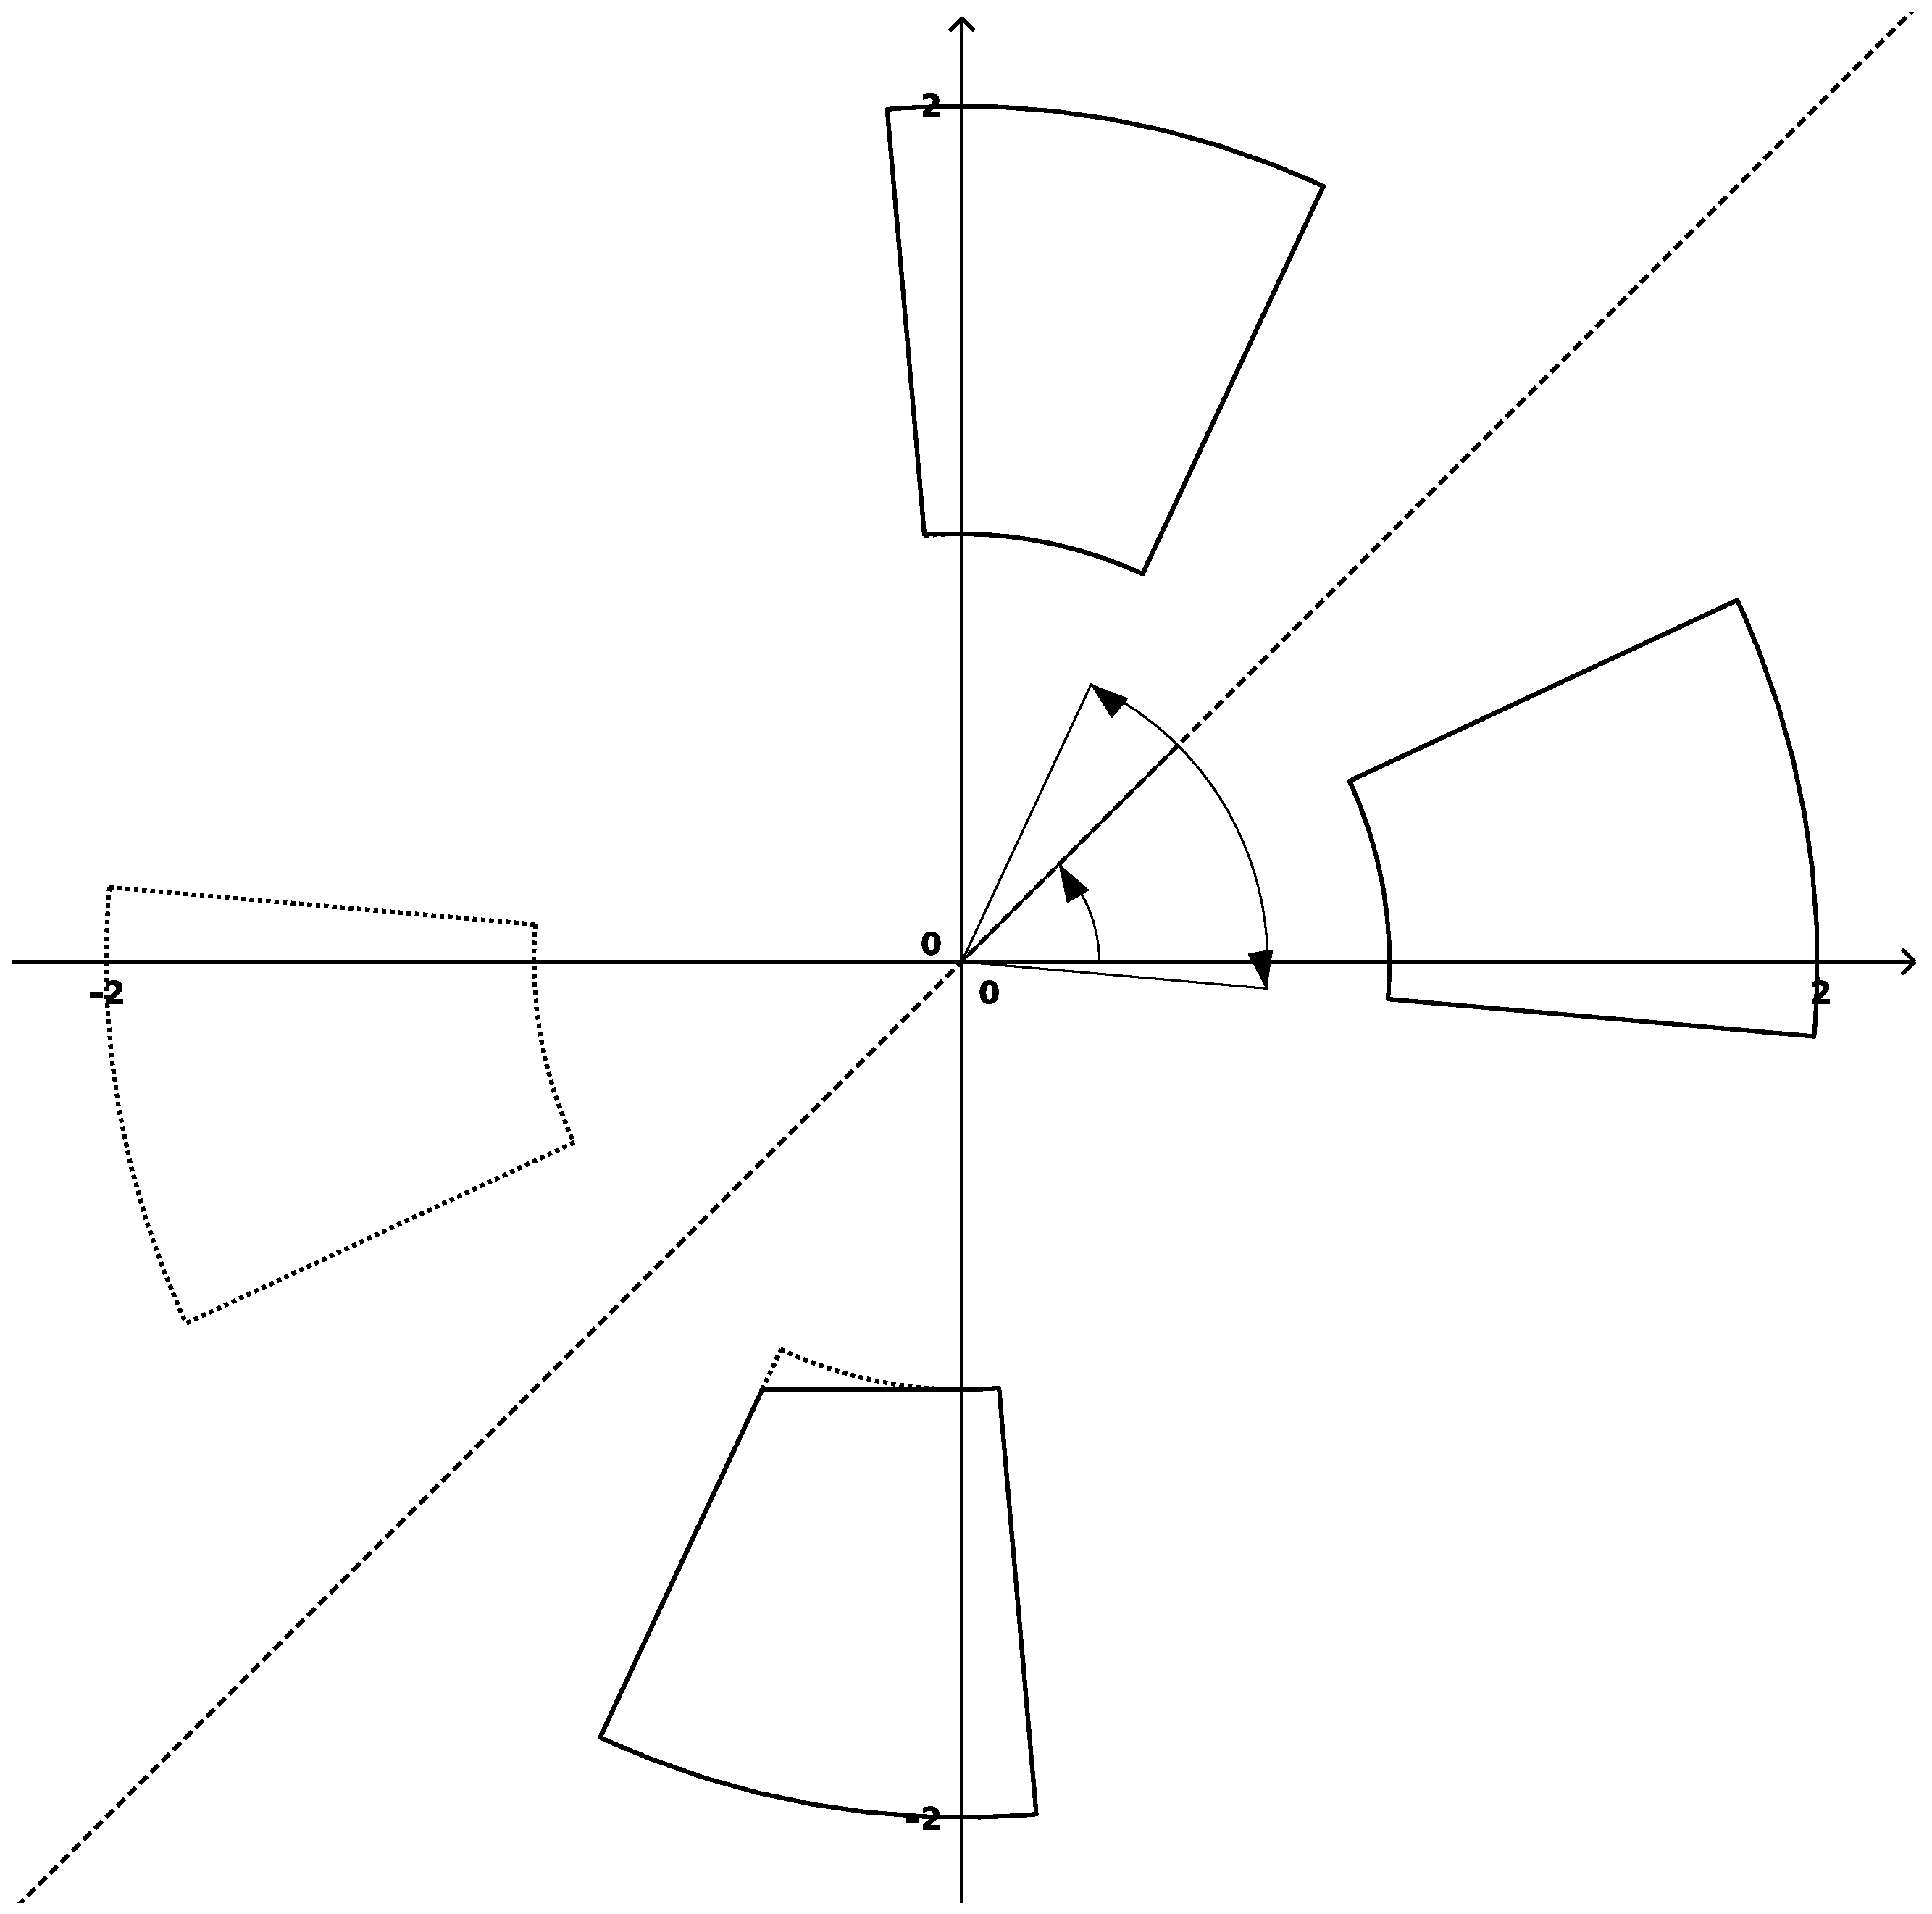
\includegraphics[width=0.5\textwidth]{2d}
    \caption{Центральное сечение области.}
\end{figure}

\section{Поле скоростей}

В работе рассматривается две возможности задания поля скоростей. Это сферически симметричная аккреция или сферически симметричный ветер. Также учитывается вращение. Для лучевой компоненты вращения можно записать

\begin{equation}
v_{rz} = \omega_xy - \omega_yx
\end{equation}

Теперь в общем случае можно записать

\begin{equation}
v_z = v_{rz} + v_{mz}
\end{equation}

Рассмотрим отдельно ветер и аккрецию

\subsection{Аккреция}

Для лучевой компоненты сферически симметричной аккреции можно записать

\begin{equation}
v_{mz} = v_{esc}\sqrt{\left(\frac{1}{r} - \frac{1}{r_0}\right)}\ \frac{z}{r}
\end{equation}

Здесь радиус звезды взят за единицу.

Ниже приводятся контурные графики $v_{mz}$ в зависимости от $z$ и $r = x^2+y^2$. Можно заметить, что на луче $r = const$ некоторые значения скоростей встечаются дважды, что может сильно влиять на профили. 

\begin{figure}[h]
    \centering
    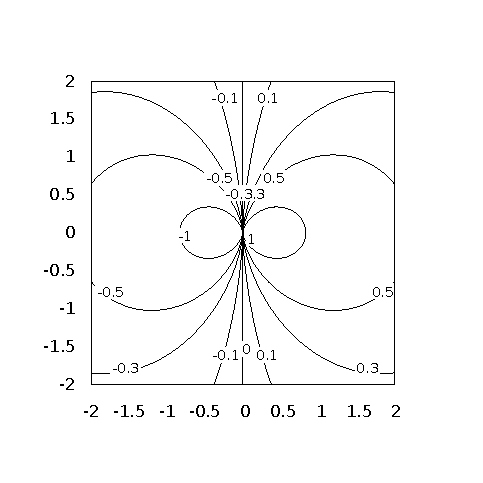
\includegraphics[width=0.49\textwidth]{plot5}
    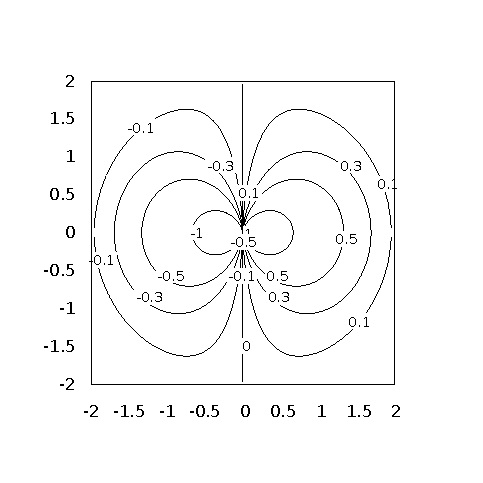
\includegraphics[width=0.49\textwidth]{plot2}
    \caption{$v_{mz}/v_{esc}$ для аккреции с $r_0=5$ и $r_0=2$.}
\end{figure}

\subsection{Ветер}

Для ветра используется классическое выражение из \cite{castor79}

\begin{equation}
v_{mz} = -\left(v_0 + \left(v_{\infty} - v_0\right)\left(1 - \frac{1}{r}\right)^\beta\right)\frac{z}{r}
\end{equation}

Радиус звезды также взят за единицу. За $v_0$ можно взять тепловую скорость.

\section{Расчет профиля линии}

В общем случае профиль линии задается формулой

\begin{equation}
I_{\nu} = \int \limits_{S} I_{xy}(\nu) dS
\end{equation}

Где $S$ - площадь проекции области, в которой происходит излучение, на плоскость $XY$ (ось $z$ направлена на наблюдателя) 

Рассмотрим $I_{xy}$
\begin{equation}
I_{xy}(\nu) =  \int \limits_{z_0}^{z_k} S_{ul}k_{lu}e^{-\tau}dz
\end{equation}
\begin{equation}
\tau = \int \limits_z^{z_k} k_{lu}dz
\end{equation}
\begin{equation}
S_{ul} = \frac{2h\nu_0^3}{c^2}\left(\frac{n_l}{n_u} \frac{g_u}{g_l} - 1 \right)^{-1}
\end{equation}
\begin{equation}
k_{lu} = 0,02654f_{lu}\alpha(\nu, z)n_l\left(1 - \frac{g_l}{g_u}\frac{n_u}{n_l}\right)
\end{equation}
\begin{equation}
\alpha(\nu, z) = \frac{1}{\sqrt{\pi} \Delta\nu_D} \exp\left( -\left[ \frac{\nu}{\Delta\nu_D} - \frac{v_z(z)}{u}\right]^2\right)
\end{equation}

Где $S(z)$ - функция источника, $k(\nu, z)$ - коэффициент поглощения, $\nu_0$ - центральная частота линии, $u$ - тепловая скорость, $\Delta\nu_D$ - доплеровская ширина линии, $v_z(z)$ - лучевая скорость вещества в точке $(x, y, z)$.

Населенности уровней задаются извне. 

Излучение в континууме задается формулой Планка.

\begin{equation}
I_c = \frac{2h\nu^3}{c^2}\frac{1}{\exp\left(\frac{h\nu}{k_bT_s}\right)-1}
\end{equation}

Где $T_s$ - эффективная температура звезды. Теперь можно рассчитать профиль $r_{\nu}$

\begin{equation}
r_{\nu} = \frac{I_\nu + I_{\tau}(\nu)}{I_c \pi R_\ast^2}
\end{equation}

Где $I_{\tau}$ учитывает поглощение излучения звезды в области

\begin{equation}
I_{\tau}(\nu) = \int \limits_{S_\ast} I_c e^{-\tau} dS
\end{equation}

Где $S_\ast$ - проекция звезды на картинную плоскость, а $\tau$ - оптическая толщина на всем луче.

\section{Параметры модели}

Подведя итог всего выше сказанного можно сказать, что для расчета профиля линии нужны 11 параметров: температура звезды, радиус звезды, 5 углов, задающих область, внешний радиус области, температура газа в области, угловая скорость вращения звезды, а также два параметра для поля скоростей ($\beta$ и $v_{\infty}$ для ветра или $v_{esc}$ и $r_0$ для аккреции). Ниже приводятся результаты для различных моделей.

\section{Результаты}

Были рассчитаны профили линий для аккреции и ветра при отсутствии ЛТР. Расчеты населенностей были выполнены Л.В.Тамбовцевой в приближении Соболева, с использованием алгоритма, описанного в работах Гринина и Катышевой \cite{grinin80} и Гринина и Мицкевича \cite{grinin90}.

\subsection{Ветер}

Ниже приводятся рассчитанные профили линий $H_\alpha$ и $H_\beta$ для ветра (Рис. 4). В моделях использовались две конфигурации области: с углами расвора 60 и 90 (что можно использовать для моделирования дискового ветра) и 30, 60 (что можно использовать для X-ветра). Параметры модели (в том числе и параметры, использованные для расчета населенностей уровней): температура звезды и газа (8000K и 10000К), $v_\infty$ (400 км/с), $beta$ (3.0), радиус области (10 $R_\ast$), радиус звезды (2.6 $R_\odot$), угловая скорость звезды (30 км/с на экваторе), углы $\psi$ и $\alpha$ (0). Ряды отличаются углом $i$. Он равен 0, 30, 45, 60, 90 градусам от верхнего к нижнему ряду графиков. Первые два столбца -- линия $H_\alpha$ для углов раствора 60, 90 и 30, 60 соответственно. Вторые два -- $H_\beta$ для тех же углов раствора. По оси абсцисс отложена $\Delta v = c(\lambda - \lambda_0) / \lambda_0 $. Далее для ветра все профили будут в таком формате. Также приводятся карты излучения (Рис. 5).

\begin{figure}
	\centering
    \includegraphics[width=0.24\textwidth]{profHa3wind06090}
    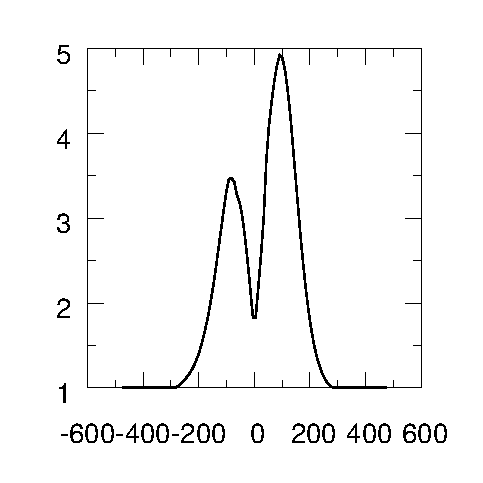
\includegraphics[width=0.24\textwidth]{profHa3wind03060}
    \includegraphics[width=0.24\textwidth]{profHb3wind06090}    
    \includegraphics[width=0.24\textwidth]{profHb3wind03060}
    
    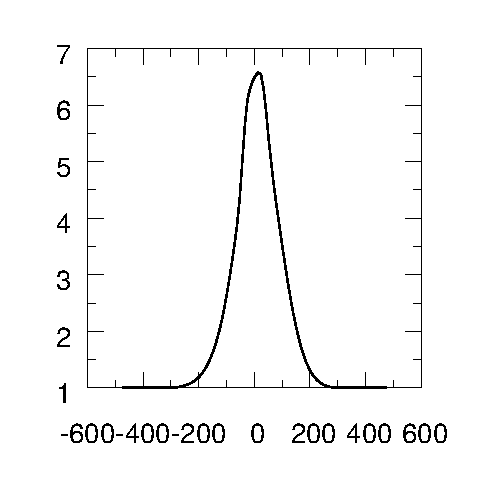
\includegraphics[width=0.24\textwidth]{profHa3wind306090}
    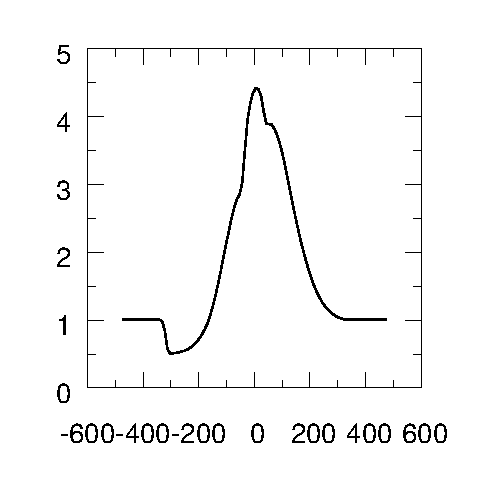
\includegraphics[width=0.24\textwidth]{profHa3wind303060}
    \includegraphics[width=0.24\textwidth]{profHb3wind306090}    
    \includegraphics[width=0.24\textwidth]{profHb3wind303060}
    
    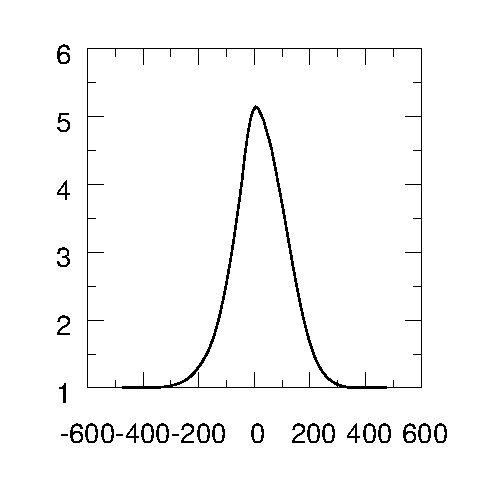
\includegraphics[width=0.24\textwidth]{profHa3wind456090}
    \includegraphics[width=0.24\textwidth]{profHa3wind453060}
    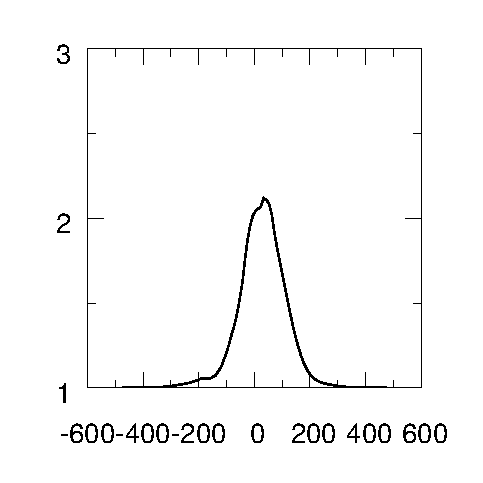
\includegraphics[width=0.24\textwidth]{profHb3wind456090}    
    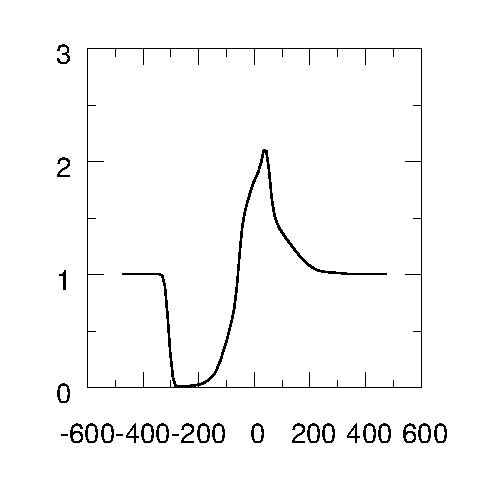
\includegraphics[width=0.24\textwidth]{profHb3wind453060}
    
    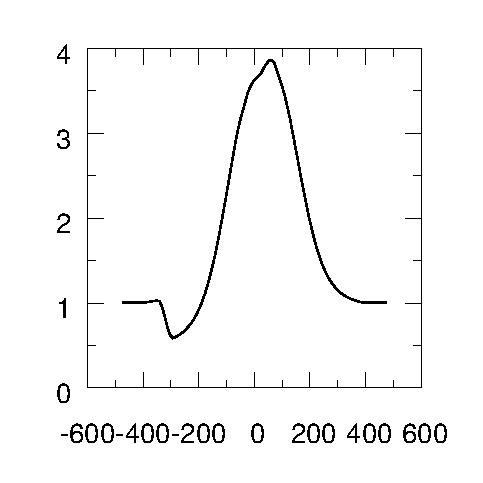
\includegraphics[width=0.24\textwidth]{profHa3wind606090}
    \includegraphics[width=0.24\textwidth]{profHa3wind603060}
    \includegraphics[width=0.24\textwidth]{profHb3wind606090}    
    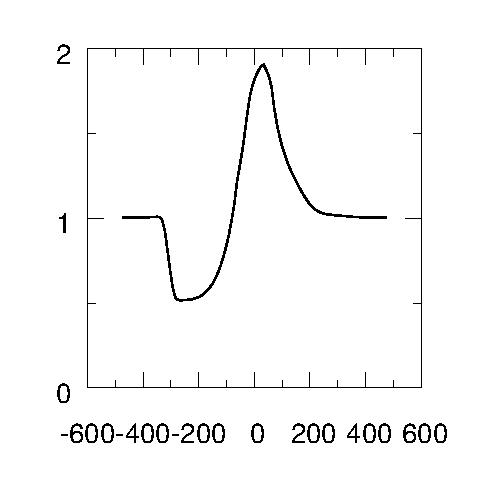
\includegraphics[width=0.24\textwidth]{profHb3wind603060}
    
    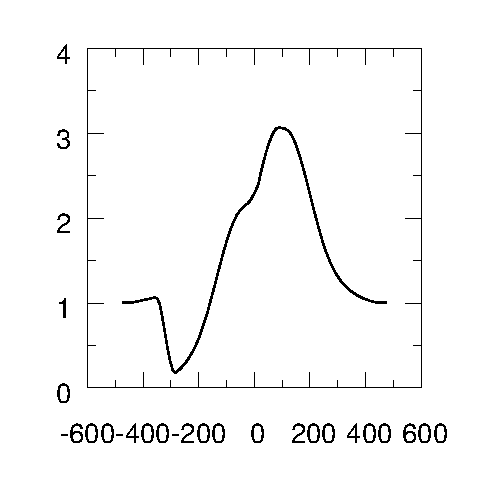
\includegraphics[width=0.24\textwidth]{profHa3wind906090}
    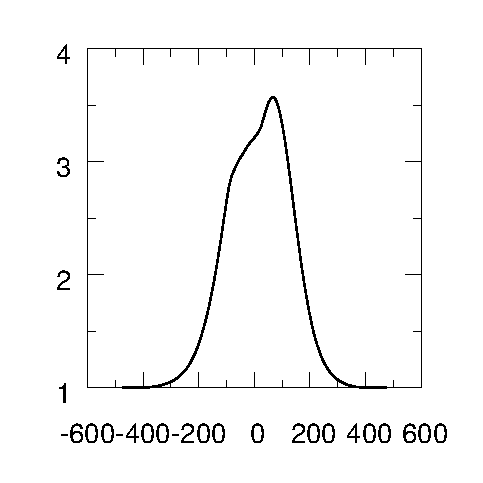
\includegraphics[width=0.24\textwidth]{profHa3wind903060}
    \includegraphics[width=0.24\textwidth]{profHb3wind906090}    
    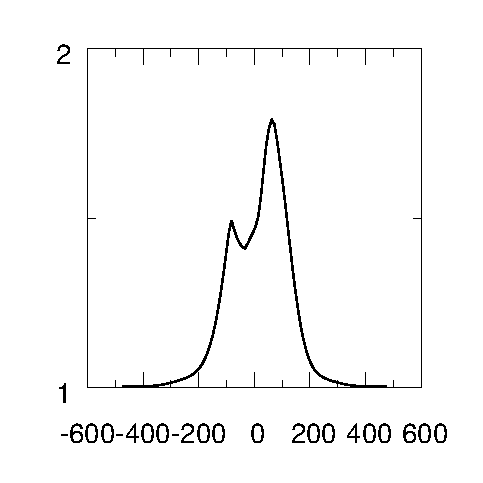
\includegraphics[width=0.24\textwidth]{profHb3wind903060}
    
    \caption{Линии $H_\alpha$ и $H_\beta$ для ветра. }
\end{figure}


\begin{figure}
	\centering
	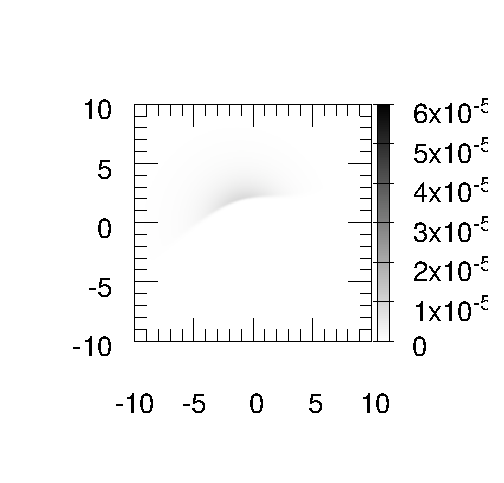
\includegraphics[width=0.24\textwidth]{map-2Ha3wind306090}
	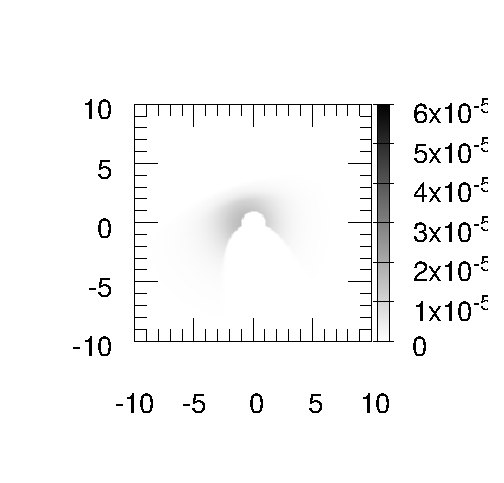
\includegraphics[width=0.24\textwidth]{map-2Ha3wind303060}
	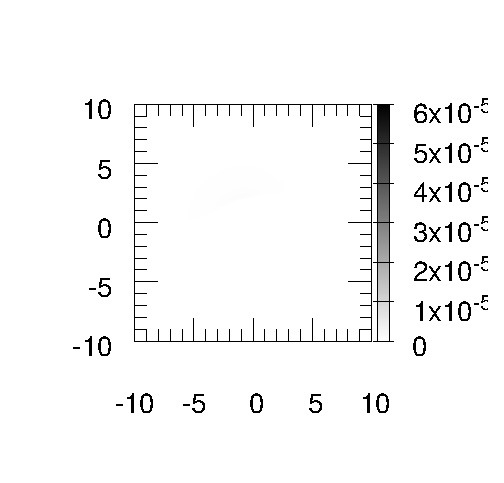
\includegraphics[width=0.24\textwidth]{map-2Hb3wind306090}
	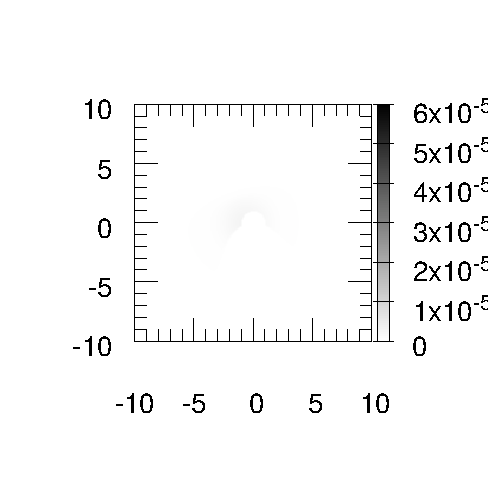
\includegraphics[width=0.24\textwidth]{map-2Hb3wind303060}
	
	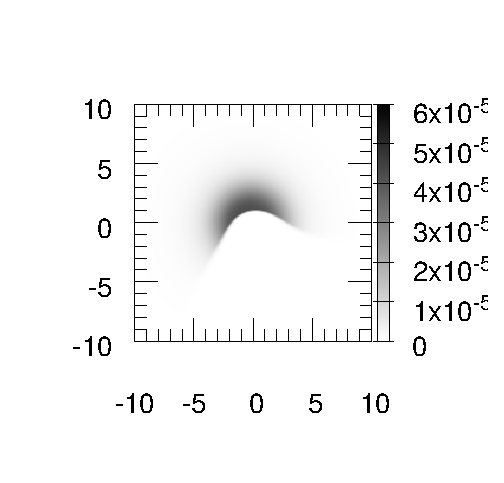
\includegraphics[width=0.24\textwidth]{map-1Ha3wind306090}
	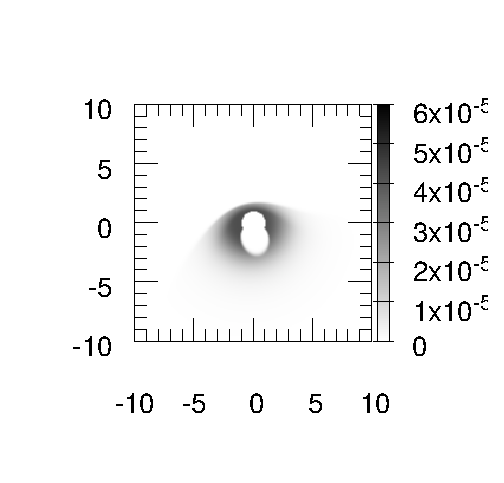
\includegraphics[width=0.24\textwidth]{map-1Ha3wind303060}
	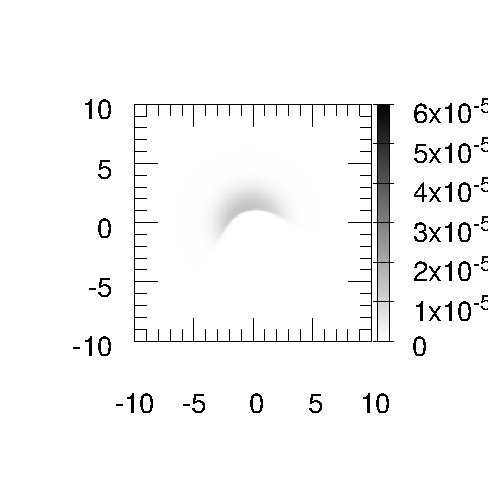
\includegraphics[width=0.24\textwidth]{map-1Hb3wind306090}
	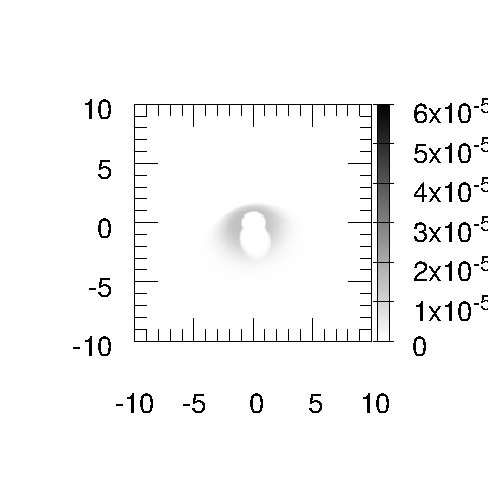
\includegraphics[width=0.24\textwidth]{map-1Hb3wind303060}
	
	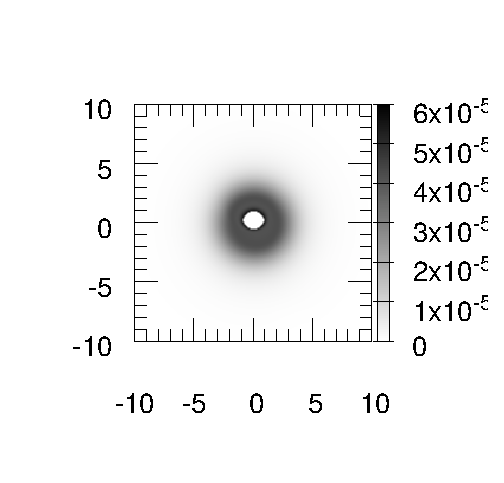
\includegraphics[width=0.24\textwidth]{map0Ha3wind306090}
	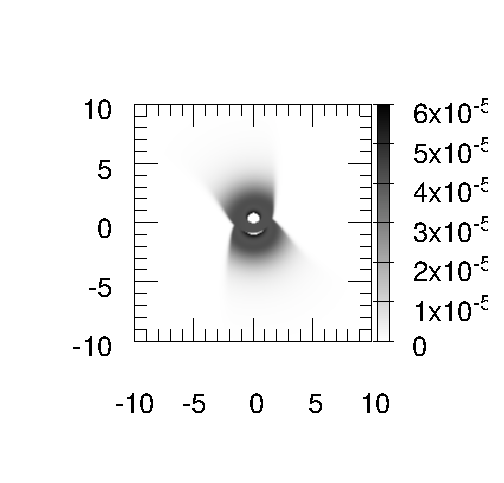
\includegraphics[width=0.24\textwidth]{map0Ha3wind303060}
	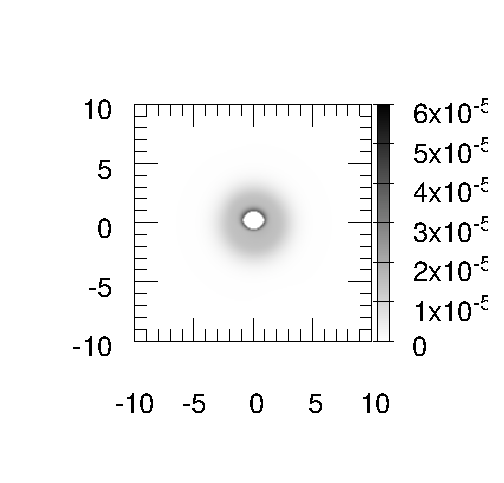
\includegraphics[width=0.24\textwidth]{map0Hb3wind306090}
	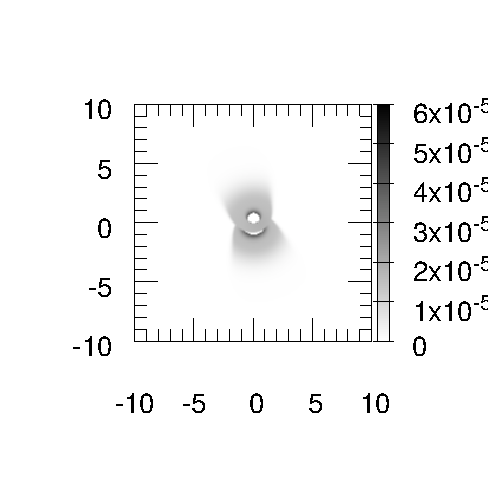
\includegraphics[width=0.24\textwidth]{map0Hb3wind303060}
	
	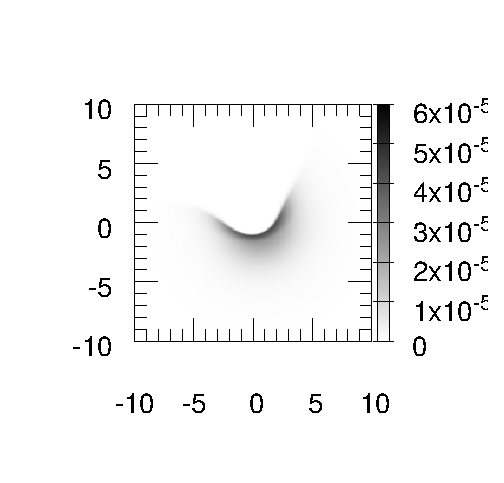
\includegraphics[width=0.24\textwidth]{map1Ha3wind306090}
	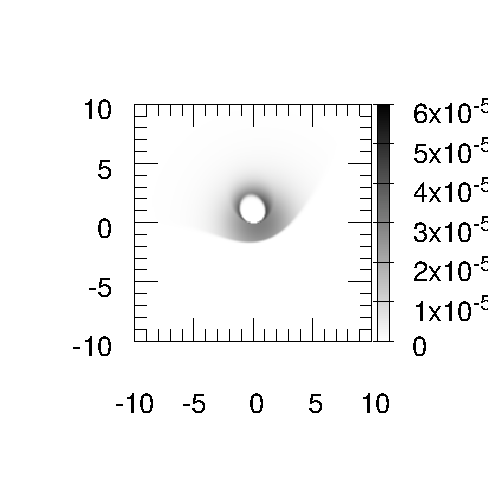
\includegraphics[width=0.24\textwidth]{map1Ha3wind303060}
	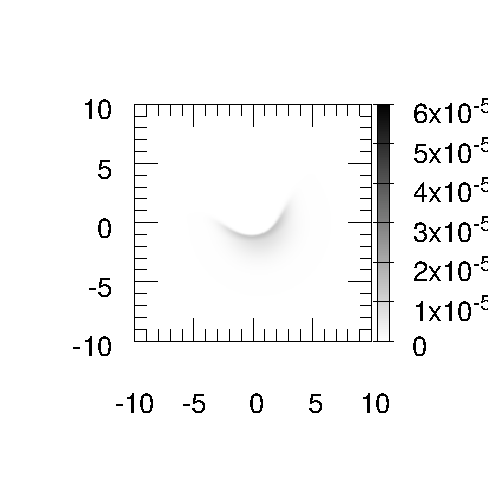
\includegraphics[width=0.24\textwidth]{map1Hb3wind306090}
	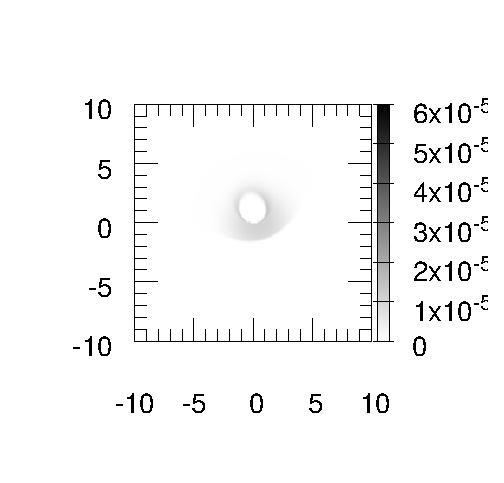
\includegraphics[width=0.24\textwidth]{map1Hb3wind303060}
	
	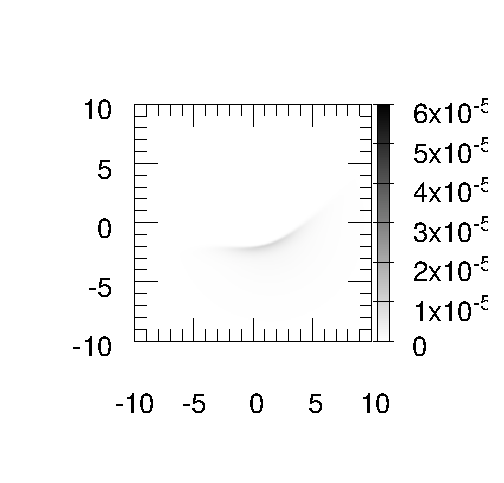
\includegraphics[width=0.24\textwidth]{map2Ha3wind306090}
	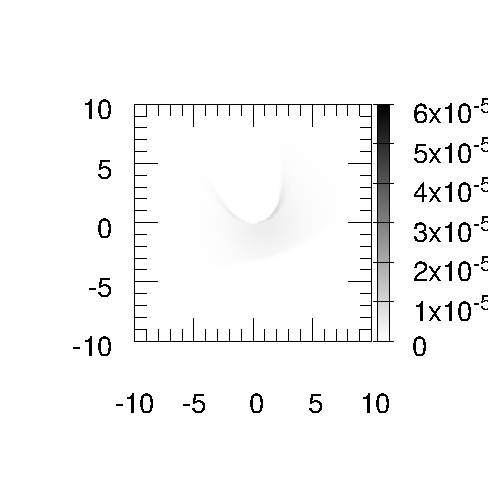
\includegraphics[width=0.24\textwidth]{map2Ha3wind303060}
	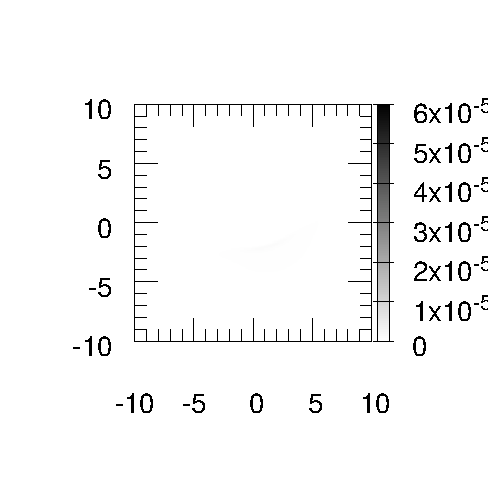
\includegraphics[width=0.24\textwidth]{map2Hb3wind306090}
	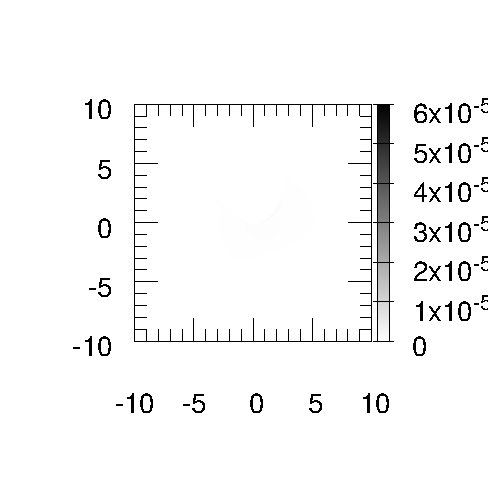
\includegraphics[width=0.24\textwidth]{map2Hb3wind303060}
	
	\caption{Карты излучения в линии $H_\alpha$ и $H_\beta$ для ветра для областей с углом наклона в 30 градусов. Столбцы отвечают за то же, что для профилей. Ряды идут от маленьких длин волн к большим (сверху вниз). Для центрального ряда $\lambda=\lambda_0$.}
	
\end{figure}
	
\subsection{Аккреция}

Также рассчитывались профили линий $H_\alpha$ и $H_\beta$ для аккреции (Рис. 6). В моделях использовалась конфигурация области с углами расвора 30 и 45. Во всех случаях неизменными оставались температура звезды и газа (8000K и 1000К), $M_\ast$ (4 $M_\odot$), радиус области (2 $R_\ast$), стартовый радиус $r_0$ (3.0 $R_\ast$), радиус звезды (2.6 $R_\odot$), угловая скорость звезды (30 км/с на экваторе), углы $\psi$ и $\alpha$ (0). Изменяемым параметром был угол наклона $i$, принимавший значения 0, 30, 45, 60, 90 градусов (на рисунке он возрастает от верхнего ряда к нижнему). Также представлены карты излучения (Рис. 7).  

\begin{figure}
	\centering
	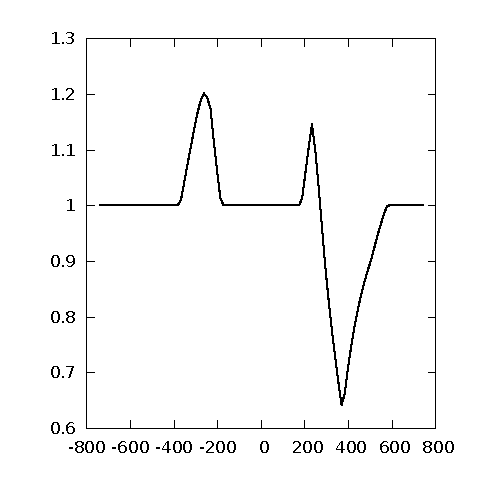
\includegraphics[width=0.3\textwidth]{profHa3accr03045}
	\includegraphics[width=0.3\textwidth]{profHb3accr03045}

	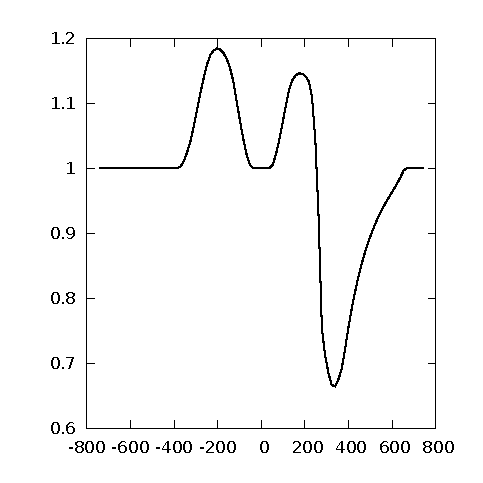
\includegraphics[width=0.3\textwidth]{profHa3accr303045}
	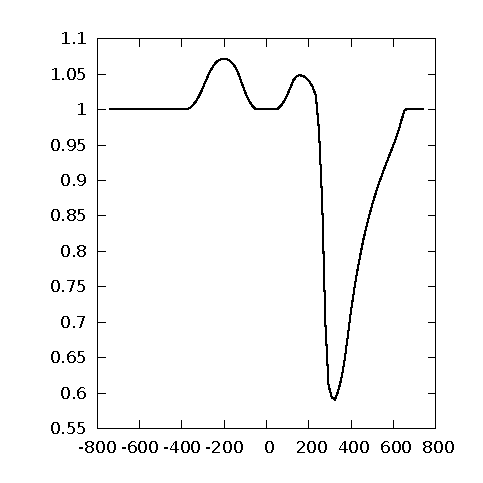
\includegraphics[width=0.3\textwidth]{profHb3accr303045}

	\includegraphics[width=0.3\textwidth]{profHa3accr453045}
	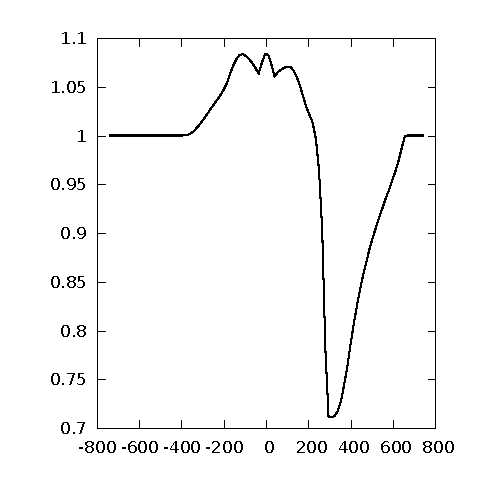
\includegraphics[width=0.3\textwidth]{profHb3accr453045}

	\includegraphics[width=0.3\textwidth]{profHa3accr603045}
	\includegraphics[width=0.3\textwidth]{profHb3accr603045}

	\includegraphics[width=0.3\textwidth]{profHa3accr903045}
	\includegraphics[width=0.3\textwidth]{profHb3accr903045}
	\caption{Профили $H_\alpha$(слева) и $H_\beta$(справа) для аккреции.}
\end{figure}

\begin{figure}
	\centering
	\includegraphics[width=0.3\textwidth]{map-2Ha3accr453045}
	\includegraphics[width=0.3\textwidth]{map-2Hb3accr453045}
	
	\includegraphics[width=0.3\textwidth]{map-1Ha3accr453045}
	\includegraphics[width=0.3\textwidth]{map-1Hb3accr453045}
	
	\includegraphics[width=0.3\textwidth]{map0Ha3accr453045}
	\includegraphics[width=0.3\textwidth]{map0Hb3accr453045}
	
	\includegraphics[width=0.3\textwidth]{map1Ha3accr453045}
	\includegraphics[width=0.3\textwidth]{map1Hb3accr453045}
	
	\includegraphics[width=0.3\textwidth]{map2Ha3accr453045}
	\includegraphics[width=0.3\textwidth]{map2Hb3accr453045}
	\caption{Карты излучения линий $H_\alpha$(слева) и $H_\beta$(справа) для аккреции. Угол $i$ равен 45 градусам.}
\end{figure}
\newpage


\begin{thebibliography}{99}
\bibitem{castor79} Castor J. I., Lamers H. J. G. L. M., 1979, ApJS, 39, 481
\bibitem{sobolev47} В.В. Соболев, Движущиеся оболочки звезд, 1947
\bibitem{petrov} П.П. Петров, Астрофизика
\bibitem{waters98} Waters, Waelkence, Ann. Rev. Astron. Astrophys. 1998 
\bibitem{hartman94} L. Hartmann et al. ApJ, 1994
\bibitem{shu94} F. Shu et al. ApJ, 1994
\bibitem{grinin11} В.П. Гринин, Л.В. Тамбовцева, Астрон. Ж. 2011
\bibitem{buve99} Бувье и др. Astron. Astrophys. 1999
\bibitem{alenkar10} Аленкар и др. Astron. J. 119, 1881, 2010
\bibitem{grinin80} В.П Гринин, Н.А. Катышева, Изв. Крымск. астрофиз. обсерв. 62, 59 (1980).
\bibitem{grinin90} В.П. Гринин, А.С. Мицкевич, Астрофизика, 32, 383 (1990).

\end{thebibliography}
\end{document}


